\documentclass[12pt, openany]{report}
\usepackage[utf8]{inputenc}
\usepackage[T1]{fontenc}
\usepackage{amsmath,amsfonts,amssymb}
\usepackage{amssymb}
\usepackage{multicol}
\usepackage[a4paper,left=2.5cm,right=2.5cm,top=2.5cm,bottom=2.5cm]{geometry}
\usepackage[english]{babel}
\usepackage{libertine}
\usepackage{graphicx}
\usepackage{wrapfig}
\usepackage{algorithm}
\usepackage{algpseudocode}
\usepackage{float}
\usepackage{enumitem}
\usepackage{pythonhighlight}
\usepackage[]{titletoc}
\usepackage{empheq}
\usepackage{titlesec}
\usepackage{mathpazo}
\usepackage{xfrac}
\usepackage{textcomp}
\usepackage{mathtools}
\usepackage{caption}
\usepackage{tabularray}
\usepackage{subcaption}
\usepackage[bottom]{footmisc}
\usepackage{pdfpages}
\usepackage{tabularx}
\usepackage{amsthm}
\usepackage[skins]{tcolorbox}
\titleformat{\chapter}[display]
  {\normalfont\bfseries}{}{0pt}{\Huge}
\usepackage{hyperref}
\newcommand{\hsp}{\hspace{20pt}}
\newcommand{\HRule}{\rule{\linewidth}{0.5mm}}
\newcommand{\R}{\mathbb{R}}
\newcommand{\C}{\mathbb{C}}
\newcommand{\E}{\mathbb{E}}
\theoremstyle{definition}
\newtheorem{thm}{Theorem}[chapter]
\newtheorem{definition}[thm]{Definition}
\newtheorem{lem}[thm]{Lemma}

\hbadness=100000
\begin{document}
\begin{titlepage}
    \begin{sffamily}
    \begin{center}
        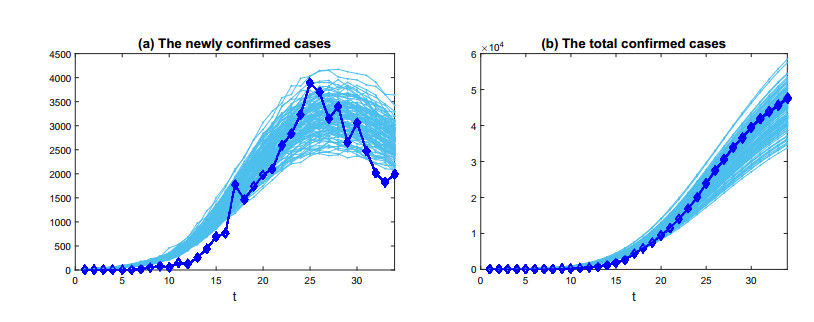
\includegraphics[scale=0.5]{img/page_de_garde.png} \\[1cm]
        \HRule \\[0.4cm]
        { \huge \bfseries LINMA2470 Stochastic Modelling \\[0.4cm] }
    
        \HRule \\[1.5cm]
        \textsc{\LARGE Simon Desmidt}\\[1cm]
        \vfill
        \vspace{2cm}
        {\large Academic year 2024-2025 - Q2}
        \vspace{0.4cm}
         
        
\includegraphics[width=0.15\textwidth]{img/epl.png}
        
        UCLouvain\\
    
    \end{center}
    \end{sffamily}
\end{titlepage}

\setcounter{tocdepth}{1}
\tableofcontents
\chapter{Reminders}
\section{General properties of probability}
\begin{itemize}
  \item $P[A\cup B]=P[A]+P[B]-P[1\cap B]$;
  \item $P[A|B] = \frac{P[A\cap B]}{P[B]} = \frac{P[AB]}{P[B]}$;
  \item $A$ and $B$ are independent iff $P[AB]=P[A]P[B]\Longrightarrow P[A|B]=P[A]$;
  \item $P[X\le x]=F_X(x)$ is the distribution function, i.e. a monotone increasing function of $x$ going from 0 to 1 when $x$ goes from $-\infty$ to $+\infty$.
  \item Its derivative is the density function $f_X(x)$ such that $f_X(x)\delta \approx P[x\le X\le x+\delta]$ for an infinitesimal $\delta$.
  \item A random variable $X$ is said to be memoryless if $\forall t,x>0$, $P[X>t+x|X>t]=P[X>x]$.
  \item Markov inequality (for a nonnegative random variable): $P[Y\ge y] \le \frac{\E[Y]}{y}$;
  \item Chebyshev inequality: $P[|Z-\E[Z]| \ge \varepsilon] \le \frac{\sigma_Z^2}{\varepsilon^2}$;
\end{itemize}
\section{Expectation and variance}
\begin{itemize}
  \item For a discrete random variable, $\E[X]= \sum_{n=-\infty}^\infty nP[X=n]$;
  \item For a continuous random variable, $\E[X]=\int_{-\infty}^\infty xf_X(x)dx$;
  \item $\E[X] = \int_0^\infty (1-F_X(x))dx$.
  \item $Var[X] = \sigma_X^2 = \E[(X-\E[X])^2] = \E[X^2] - \E[X]^2$;
\end{itemize}
\section{Law of large numbers}
Let $X_1,\dots,X_n$ be a series of independent and uniformly distributed (IID) random variables with expectation $\bar X$ and finite variance $\sigma_X^2$. Let $S_n = X_1+\dots +X_n$. Then, 
\begin{itemize}
  \item Weak version:
\end{itemize}
\begin{equation}
  \lim_{n\to \infty} P\left[|\frac{S_n}{n}-\bar X|\ge \varepsilon\right] = 0
\end{equation}
\begin{itemize}
  \item Strong version:
\end{itemize}
\begin{equation}
  \lim_{n\to \infty} P\left[\sup_{m\ge n}\left(\frac{S_m}{m}-\bar X\right)>\varepsilon\right] = 0\Longleftrightarrow \lim_{n\to \infty}\frac{S_n}{n}=X\qquad \text{with probability 1}
\end{equation}
\section{Central limit theorem}
\begin{equation}
  \lim_{n\to \infty} P\left[\frac{S_n-n\bar X}{\sqrt{n}\sigma}\le y\right] = \int_{-\infty}^y \frac{1}{\sqrt{2\pi}} e^{-\frac{x^2}{2}}dx
\end{equation}
\section{Exponential distribution}
\begin{itemize}
  \item $f_X(x)=\lambda e^{-\lambda x}$, for $x\ge 0$;
  \item $F_X(x)=1-e^{-\lambda x}$, for $x\ge 0$;
  \item $\E[X]=1/\lambda$.
  \item [$\rightarrow$] Note: the exponential distribution is memoryless.
\end{itemize}
\chapter{Poisson Processes}
A Poisson process $N(t)$ counts the number of arrivals with exponentially distributed inter-arrival times. 
\begin{equation}
  S_n = \sum_{i=1}^n X_i \qquad \qquad X_i \sim \exp(\lambda)
\end{equation}
$\forall n,t$, we have the relation $\{S_n\le t\}=\{N(t)\ge n\}$, where $S_n$ is a random variable telling at which time the $n$-th occurence appears.\\
\begin{itemize}
  \item [$\rightarrow$] Note: a Poisson process is memoryless: $P[Z_1>x]=e^{-\lambda x}$, with $Z_1$ be the duration of the time interval from $t$ until the first arrival after $t$.
\end{itemize}
For a Poisson process of rate $\lambda$, and any given $t>0$, the length of the interval from $t$ until the first arrival after $t$ is an exponentially distributed random variable. This random variable is idenpendent of both $N(t)$ and of the $N(t)$ arrival epochs before time $t$. It is also independent of $N(\tau)$, $\forall \tau \le t$.\\

Let us consider the process after $Z_1$, $Z_m$, the time until the $m$-th arrival after time $t$. It is independent of $N(t)$ and of the entier previous history of the process.\\
Let us denote $\tilde N(t,t') = N(t')-N(t)$. 
\begin{itemize}
  \item Stationary increments property: It has the same distribution as $N(t'-t)$, $\forall t'\ge t$ (stationary increments property);
  \item Independent increments property: For any sequence of times $0<t_1<\dots<t_k$, the set $\{N(t_1), \tilde N(t_1,t_2), \dots,\tilde N (t_{k-1}, t_k)\}$ is a set of independent random variables.
\end{itemize}
From the memoryless property, here is another definition of a Poisson process: \\
\begin{itemize}
  \item A Poisson process is a counting process that has the stationay and independent increment properties and such that 
\end{itemize}
\begin{equation}
  \begin{aligned}
    P[\tilde N(t, t+\delta)=0] &= 1-\lambda \delta +o(\delta)\\  P[\tilde N(t, t+\delta)=1] &= \lambda \delta +o(\delta)\\
    P[\tilde N(t, t+\delta)\ge2] &= o(\delta)
  \end{aligned}
\end{equation}
\section{\texorpdfstring{Distribution of $N(t)$}{Distribution of }}
$S_n$ is the sum $n$ IID random variables and $f_{S_n}$ is the convolution of $n$ times $f_X$:
\begin{equation}
  f_{S_n}(t) = \frac{\lambda^n t^{n}e^{-\lambda t}}{(n-1)!}
\end{equation}
From this, 
\begin{equation}\label{eq:poisson_distrib}
  P[N(t)=n-1] = \frac{(\lambda t)^{n}e^{-\lambda t}}{(n)!}
\end{equation}
and finally, 
\begin{equation}
  \E[N(t)] = \lambda t\qquad Var[N(t)] = \lambda t
\end{equation}
From equation \eqref{eq:poisson_distrib}, the Poisson process verifies the following probability conditions:
\begin{itemize}
  \item $P[\tilde N(t,t+\delta)=0]=1-\lambda \delta +o(\delta)$;
  \item $P[\tilde N(t,t+\delta)=1]=\lambda \delta +o(\delta)$;
  \item $P[\tilde N(t,t+\delta)\ge2]=o(\delta)$;
\end{itemize}
where we use a first-order approximation of the exponential term, with $o(\delta)$ its residual. As $o(\delta)$ is negligible, we can approximate the Poisson process as a Bernoulli process. 
\subsection{Combining Poisson processes}
Let $N_1(t)$ and $N_2(t)$ be tow independent Poisson processes. Let the process $N(t)=N_1(t)+N_2(t)$. We can show using the three properties above that $N(t)$ is a Poisson process with rate $\lambda_1+\lambda_2$.
\subsection{Subdividing a Poisson process}
Let $N(t)$ be a Poisson process with rate $\lambda$. We split the arrivals in 2 subprocesses $N_1(t)$ and $N_2(t)$. Each arrival of $N(t)$ is sent to $N_1(t)$ with probability $p$ and to $N_2(t)$ with probability $(1-p)$, each split being independent from all others. \\
Then, the resulting processes $N_1(t)$ and $N_2(t)$ are two independent Poisson processes with respective rate $p\lambda$ and $(1-p)\lambda$.
\subsection{Conditional arrival distribution}
The density probability function when we have $n$ Poisson processes, under the condition that $N(t)=n$, is
\begin{equation}
  f(s_1,\dots,s_n|N(t)=n)=\frac{n!}{t^n}
\end{equation}
From the previous results, we can compute that 
\begin{equation}
  P[S_1>\tau|N(t)=n]=\left(\frac{t-\tau}{t}\right)^n
\end{equation}
and the expectation is 
\begin{equation}
  E[S_1|N(t)=n] = \frac{t}{n+1}
\end{equation}
And from this, we derive that 
\begin{equation}
  P[X_i>\tau|N(t)=n] = \left(\frac{t-\tau}{t}\right)^n
\end{equation}
with expectation 
\begin{equation}
  E[X_i] = \frac{t}{n+1}
\end{equation}
And thus the density function is 
\begin{equation}
  f_{S_i}(x|N(t)=n) = \frac{x^{i-1}(t-x)^{n-i}n!}{t^n (n-i)!(i-1)!}
\end{equation}
\section{Non-homogenous Poisson processes}
A non-homogenous Poisson rocess $N(t)$ is a counting process with increments that are independent but not stationary, with
\begin{itemize}
  \item $P[\tilde N(t,t+\delta)=0]=1-\lambda (t)\delta + o(\delta)$;
  \item $P[\tilde N(t,t+\delta)=1]=\lambda (t)\delta + o(\delta)$;
  \item $P[\tilde N(t,t+\delta)\ge2]=o(\delta)$;
\end{itemize}
where $\tilde N(t,t+\delta)=N(t+\delta)-N(t)$. The time-varying arrival rate $\lambda(t)$ is assumed to be continuous and stricly positive.
\section{Bernoulli process approximation}
We can approximate the non-homogenous Poisson process with a Bernoulli process where the time is partitioned into increments of lengths inversely proportional to $\lambda (t)$ (i.e. using a nonlinear time scale).
\begin{itemize}
  \item $P[\tilde N(t,t+\epsilon/\lambda(t))=0]=1-\epsilon + o(\epsilon)$;
  \item $P[\tilde N(t,t+\epsilon/\lambda(t))=1]=\epsilon + o(\epsilon)$;
  \item $P[\tilde N(t,t+\epsilon/\lambda(t))\ge2]=o(\epsilon)$;
\end{itemize}
Letting $\epsilon$ tend to zero, we obtain
\begin{equation}
  P[N(t)=n]=\frac{(m(t))^ne^{-m(t)}}{n!}\qquad P[\tilde N(t,t')=n]=\frac{(m(t,t'))^n e^{-m(t,t')}}{n!}
\end{equation}
with 
\begin{equation}
  m(t)=\int_0^t \lambda(\tau)d\tau \qquad m(t,t')=\int_t^{t'} \lambda(\tau)d\tau 
\end{equation}
\section{Classification of queueing systems}
\begin{itemize}
  \item We note $A/B/k$ where $A$ is the type of distribution for the arrival process, $B$ for the service time and $k$ the number of servers.
\end{itemize}
We suppose that the arrivals wait in a single queue.
Commonly used letters are 
\begin{itemize}
  \item M: exponential distribution (for A) or Poisson process (for B);
  \item D: deterministic time intervals;
  \item E: Erlang distribution;
  \item G: general distribution.
\end{itemize}
\chapter{Renewal Processes}
A renewal process is a counting process with IID interarrival intervals. We note $X_i$ the interval between arrivals, $\bar X=\E[X]$ is supposed to be finite with probability $P[X_i]>0=1$\footnote{A probability of 1 means that the opposite can happen, but is so rare that the probability is 0.}, $\sigma$ can be finite, and we denote $S_n=\sum_{i=1} X_i$ the time of the $n$-th arrival.\\
\section{Strong law of large numbers}
Let $\{N(t);t\ge 0\}$ be a renewal process, then 
\begin{equation}
  \lim_{t\to \infty} N(t) = \infty \qquad \qquad \lim_{t\to \infty} \E[N(t)] = \infty 
\end{equation}
This implies that 
\begin{equation}
  \lim_{t\to \infty} \frac{N(t)}{t} = \frac{1}{\bar X} \text{ with probability 1}
\end{equation}
\section{Central limit theorem}
If the interarrival intervals of the renewal process $N(t)$ have a finite standard deviation, then from the CLT for IID random variables, we have 
\begin{equation}
  \lim_{t\to \infty} P\left[\frac{S_n-n\bar X}{\sqrt{n}\sigma}\le \alpha\right] = \Phi(\alpha)
\end{equation}
\textcolor{red}{What is $\Phi(\alpha)$?}\\
and 
\begin{equation}
  \lim_{t\to \infty} P\left[\frac{N(t)-t/\bar X}{\sigma \bar X^{-3/2}\sqrt{t}}<\alpha \right] = \Phi(\alpha)
\end{equation}
\begin{itemize}
  \item [$\to$] Note: The reliability of the observed mean of successive results that are supposed to be IID depends a lot on the rule used to decide when we stop repeating the experiment.
\end{itemize}
\section{Stopping time}
Let $N$ be the rv corresponding to the total number of experiments observed. Let $I_n$ be a series of rv being the indicator fucnction of $\{N\ge n\}$:
\begin{equation}
  I_n = \begin{cases}
    1 & \text{if the $n$-th experiment is observed}\\
    0 & \text{otherwise}
  \end{cases}
\end{equation}
$N$ is a stopping time if $I_n$ depends only on $X_1,\dots,X_{n-1}$. This means that stopping at 3pm, for example, is not a stopping time, because it can depend on $X_n$, depending if the $n$-th arrival is before or after 3pm.\\
\subsection{Wald's inequality}
Let $N$ be a stopping time for $\{X_n;n\ge 1\}$. Then, $\E[S_N]=\E[N]\bar X$.
\section{Blackwell's renewal theorem}
\subsection{Arithmetic distribution}
If interarrival intervals can only have a length that is a multiple of some real number $d$, the interarrival distribution will be called an arithmetic distribution, and $d$ the span of the distribution. 
\subsection{Blackwell's inequality}
If the interarrival distribution of a renewal process $N(t)$ is not arithmetic, then 
\begin{equation}
  \lim_{t\to\infty } \left(m(t+\delta)-m(t)\right) = \frac{\delta}{\bar X} \qquad \forall \delta 
\end{equation}
If the interarrival distribution is arithmetic with span $d$, then 
\begin{equation}
  \lim_{t\to\infty } \left(m(t+nd)-m(t)\right) = \frac{nd}{\bar X} \qquad \forall n\ge 1
\end{equation}
\subsection{Relationship with a Poisson process}
The sum of many renewal processes tends to a Poisson process: for a non-arithmetic renewal process with $P[X_i=0]=0$, we have 
\begin{equation}
  \begin{aligned}
    &\lim_{t\to\infty} P[N(t+\delta)-N(t)=0]=1-\delta/\bar X + o(\delta)\\
    &\lim_{t\to\infty} P[N(t+\delta)-N(t)=1]=\delta/\bar X + o(\delta)\\
	&\lim_{t\to\infty} P[N(t+\delta)-N(t)\ge 2]=o(\delta)
  \end{aligned}
\end{equation}
The increments are asymptotically stationary, but not independent. 
|section{Renewal reward process}
Along to the renewal process $N(t)$, we can add a reward function $R(t)$. It models the rate at which the process is accumulating a reward or cost. It can however only depend on the current renewal but not the previous ones. \\
Let $Y(y)$ be the residual life at time $t$ for the current renewal:
\begin{equation}
	R(t)=Y(t)=S_{N(t)+1}-t
\end{equation}
\begin{figure}[H]
	\centering
	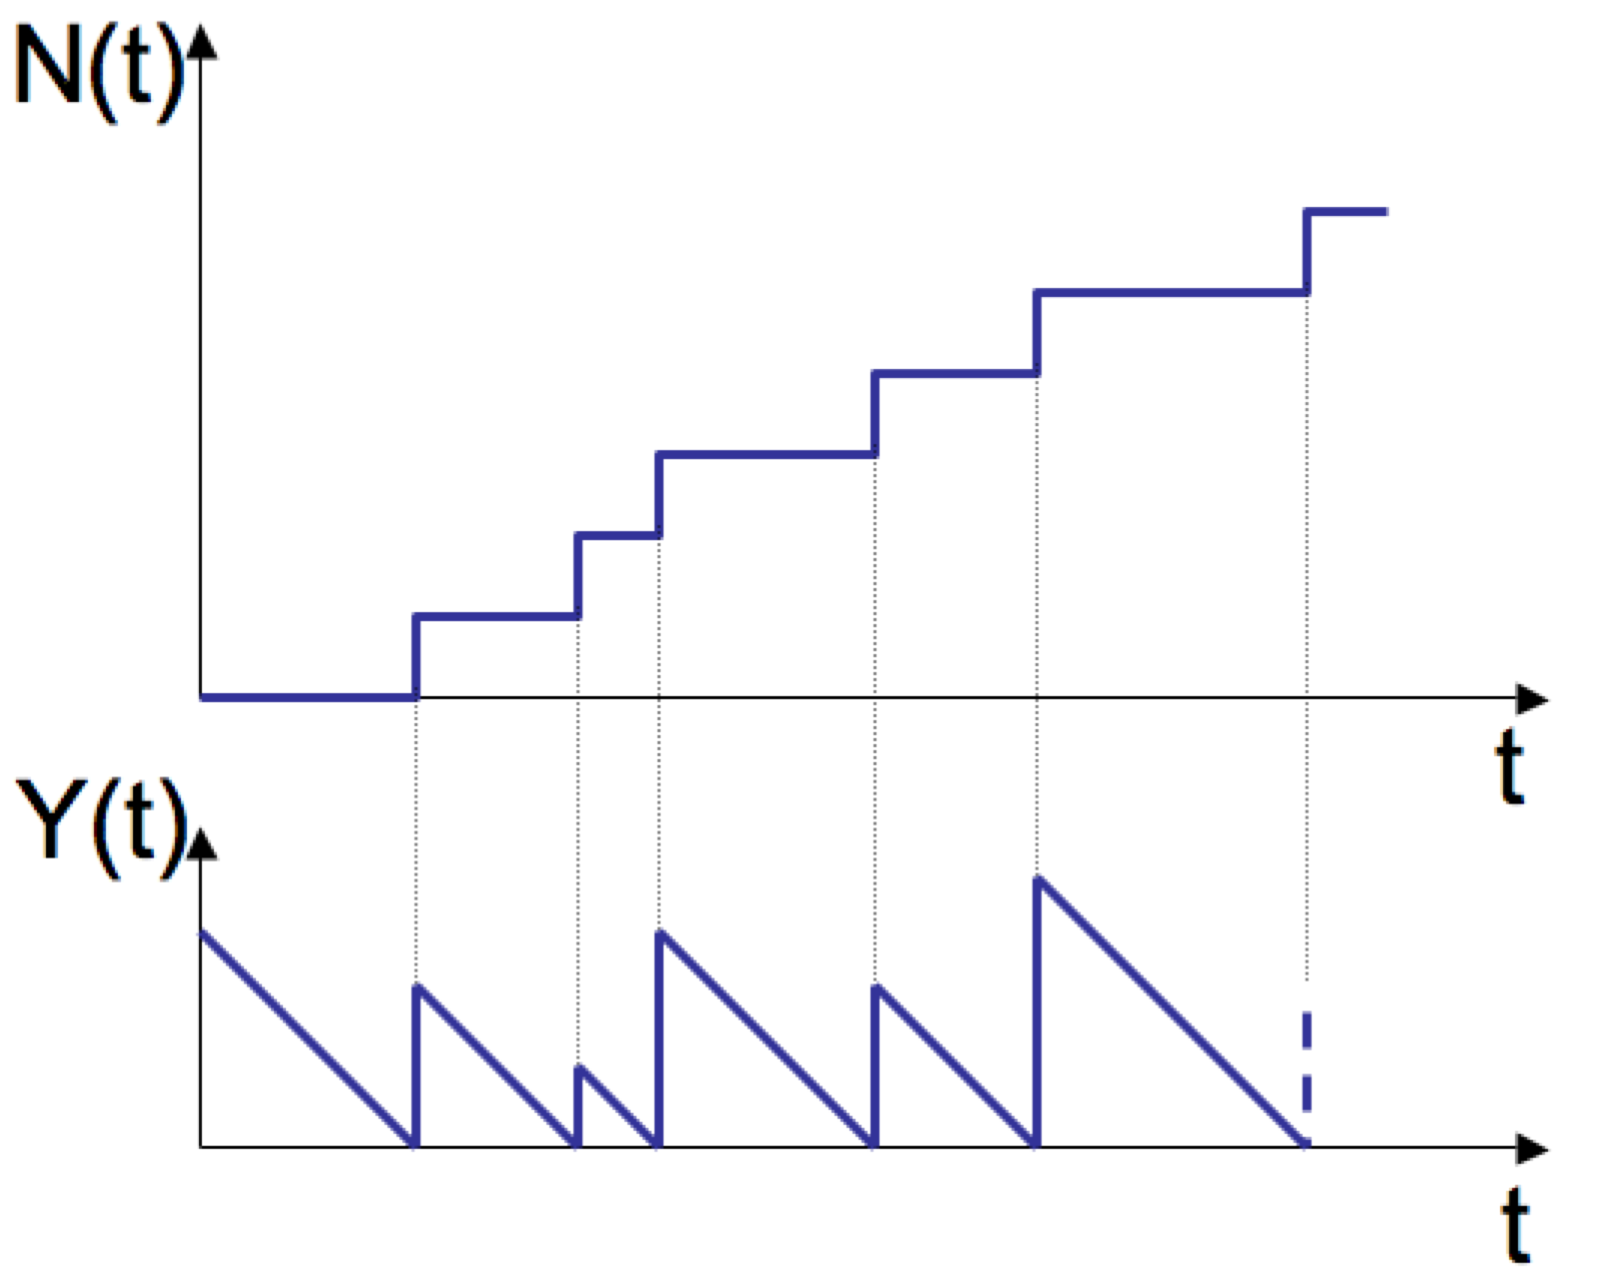
\includegraphics[width=0.5\textwidth]{img/reward.png}
\end{figure}
The time average residual life is $\frac{1}{t}\int_0^t Y(\tau)d\tau$.\\
From the definition of $Y(t)$, we can calculate that 
\begin{equation}
	\lim_{t\to \infty} \frac{1}{t}\int_0^t Y(\tau)d\tau = \frac{\E[X^2]}{2\E[X]} = \frac{1}{2}\E[X] + \frac{Var(X)}{\E[X]} > \frac{1}{2}\E[X]\text{ with probability 1}
\end{equation}
\subsection{Time average age}
Let $Z(t)$ be the age of the current renewal at time $t$: $R(t)=Z(t)=t-S_{N(t)}$. The time average age is $\lim_{t\to \infty} \frac{1}{t}\int_0^t Z(\tau)d\tau= \frac{\E[X^2]}{2\E[X]}$.\\
\begin{figure}[H]
	\centering
	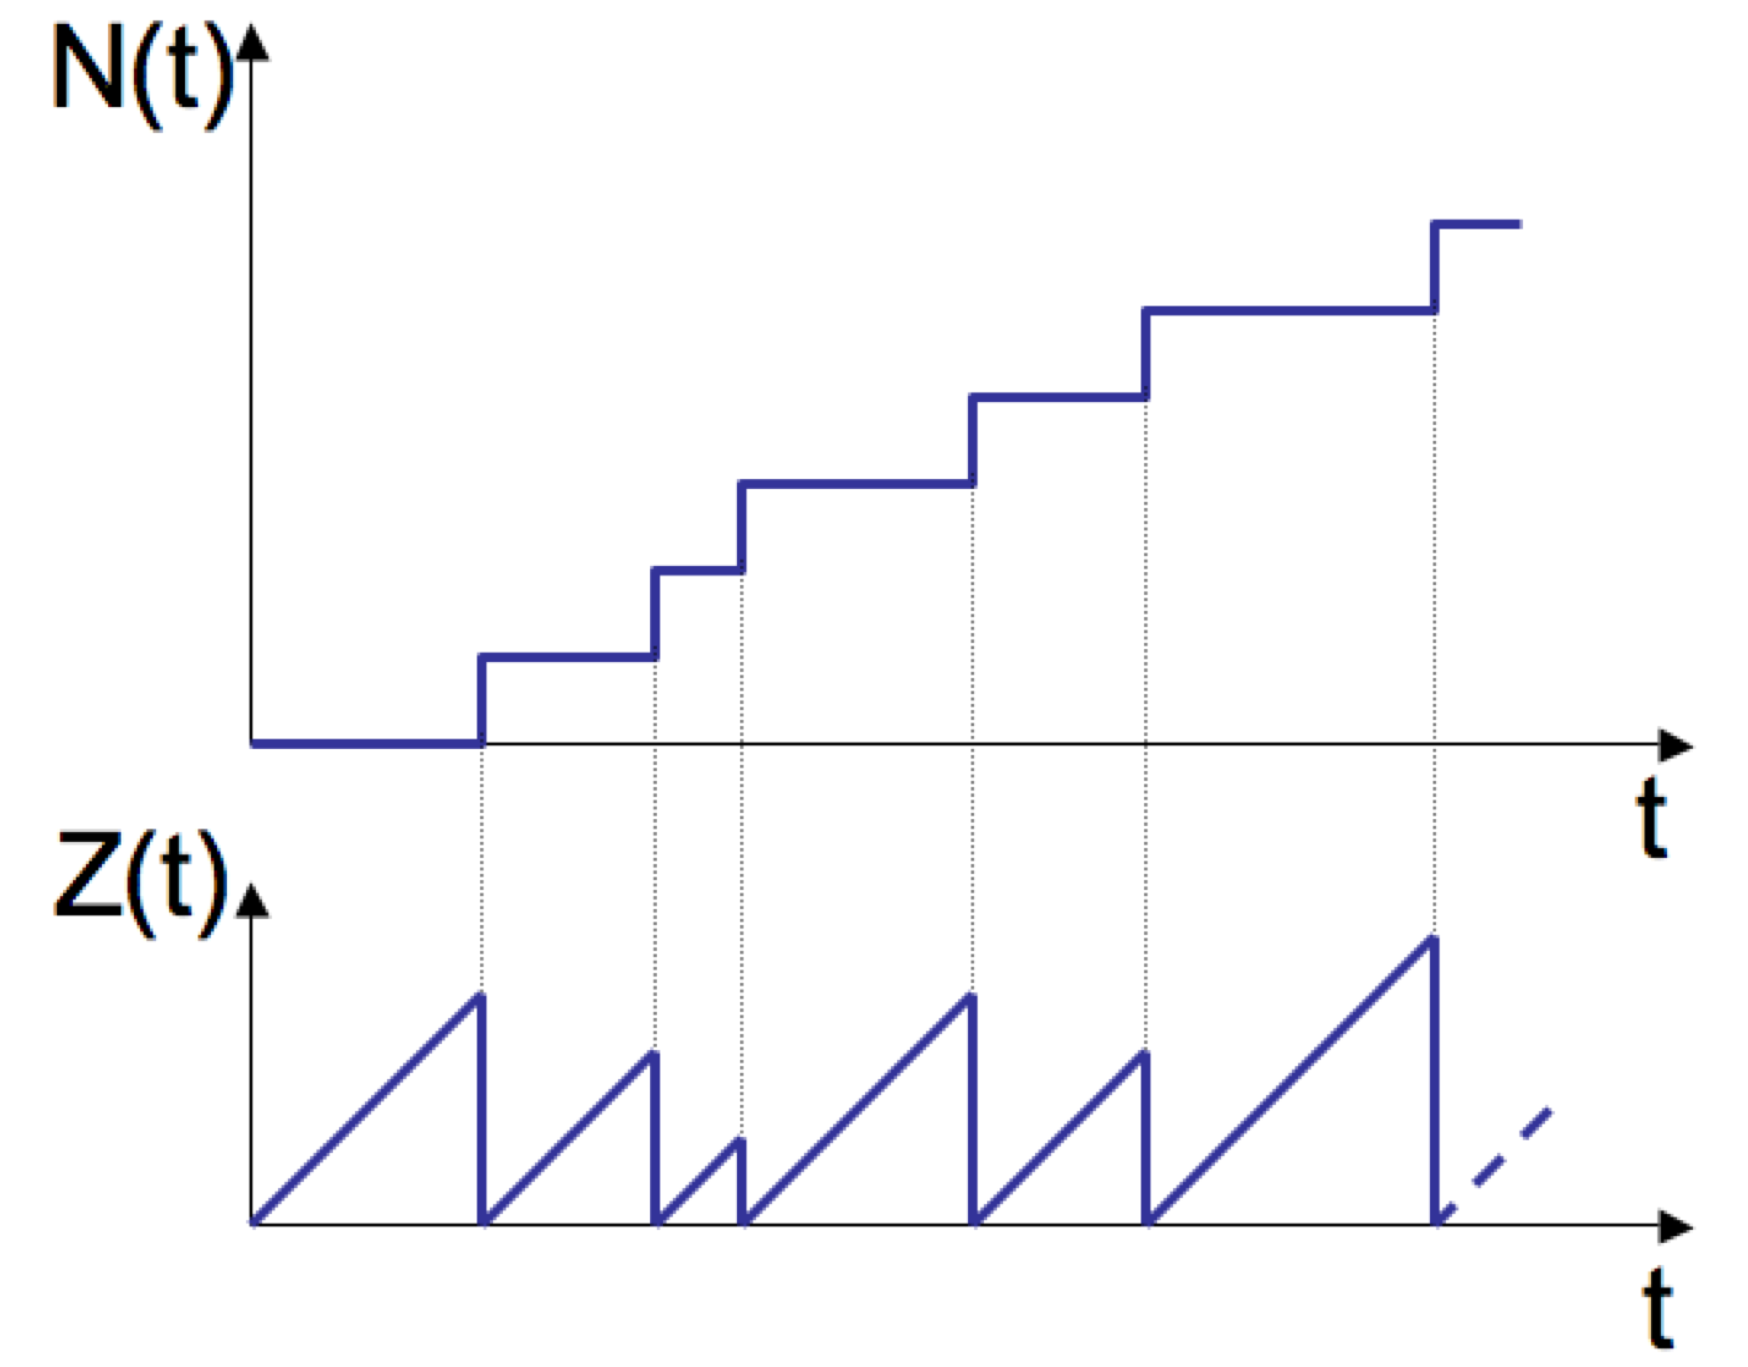
\includegraphics[width=0.5\textwidth]{img/age.png}
\end{figure}
\subsection{Time average duration}
Let $X(t)$ be the duration of the renewal containing time $t$: $R(t)=X(t)=S_{N(t)+1}-S_{N(t)}$. The time average duration is $\lim_{t\to \infty} \frac{1}{t}\int_0^t X(\tau)d\tau = \frac{\E[X^2]}{\E[X]}$.\\
\begin{figure}[H]
	\centering
	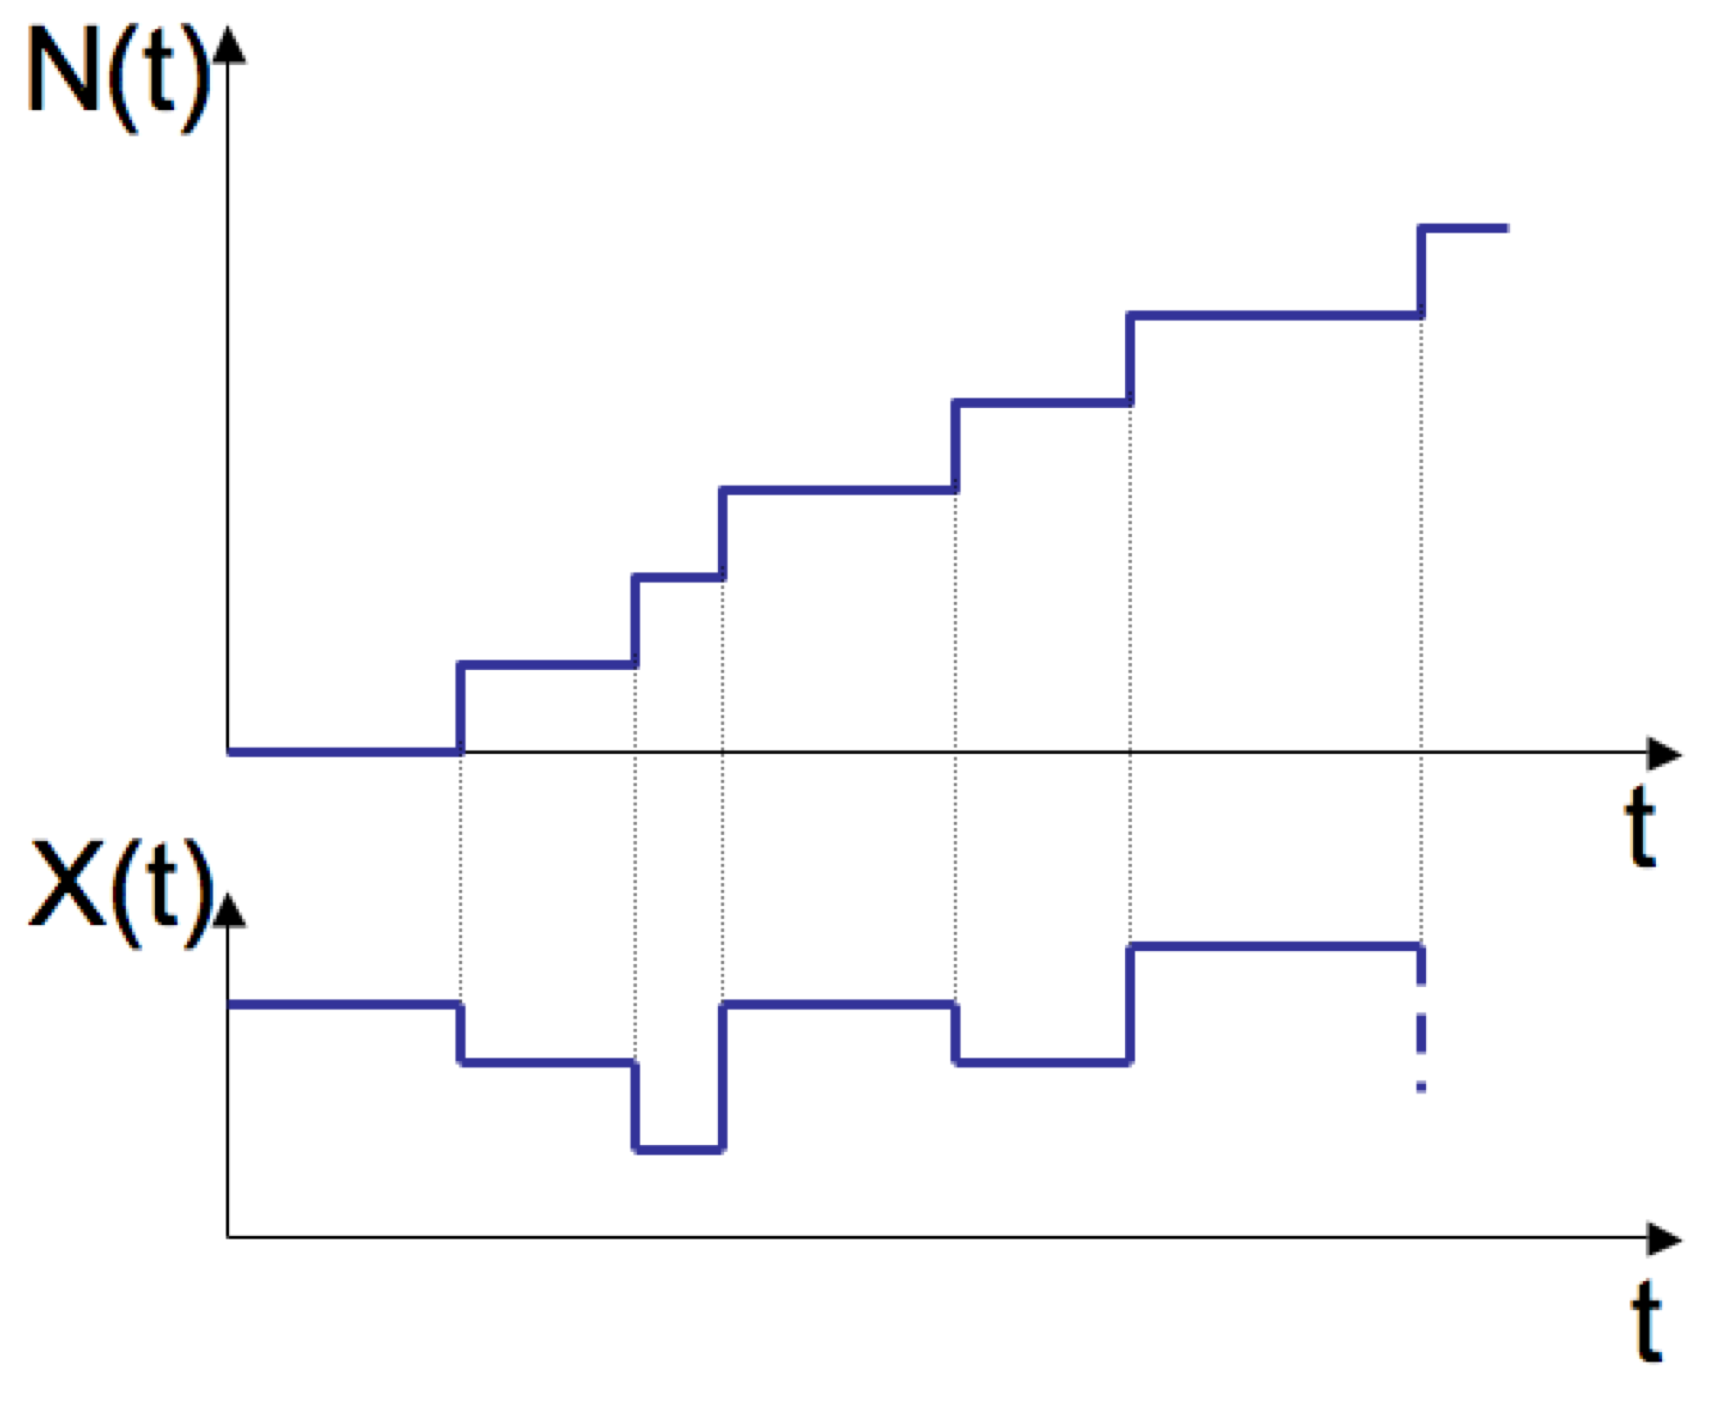
\includegraphics[width=0.5\textwidth]{img/duration.png}
\end{figure}
|subsection{General renewal reward functions}
Let $R(t)$ be a reward function for a renewal process with expected inter-renewal times $\bar X<\infty$, then with probability 1, 
\begin{equation}
	\lim_{t\to \infty} \frac{1}{t}\int_0^t R(\tau)d\tau = \frac{\E[R_n]}{\E[X]}
\end{equation}
where $R_n$ is defined as 
\begin{equation}
	R_n = \int_{S_n}^{S_{n+1}} R(\tau)d\tau
\end{equation}
\subsection{Distribution of residual life}
We are interested in the fraction of time that $Y(t)\le y$: 
\begin{equation}
	R(t)= I\{Y(t)\le y\} \qquad \qquad R_n = \min\{y, X_n\}
\end{equation}
\begin{figure}[H]
	\centering
	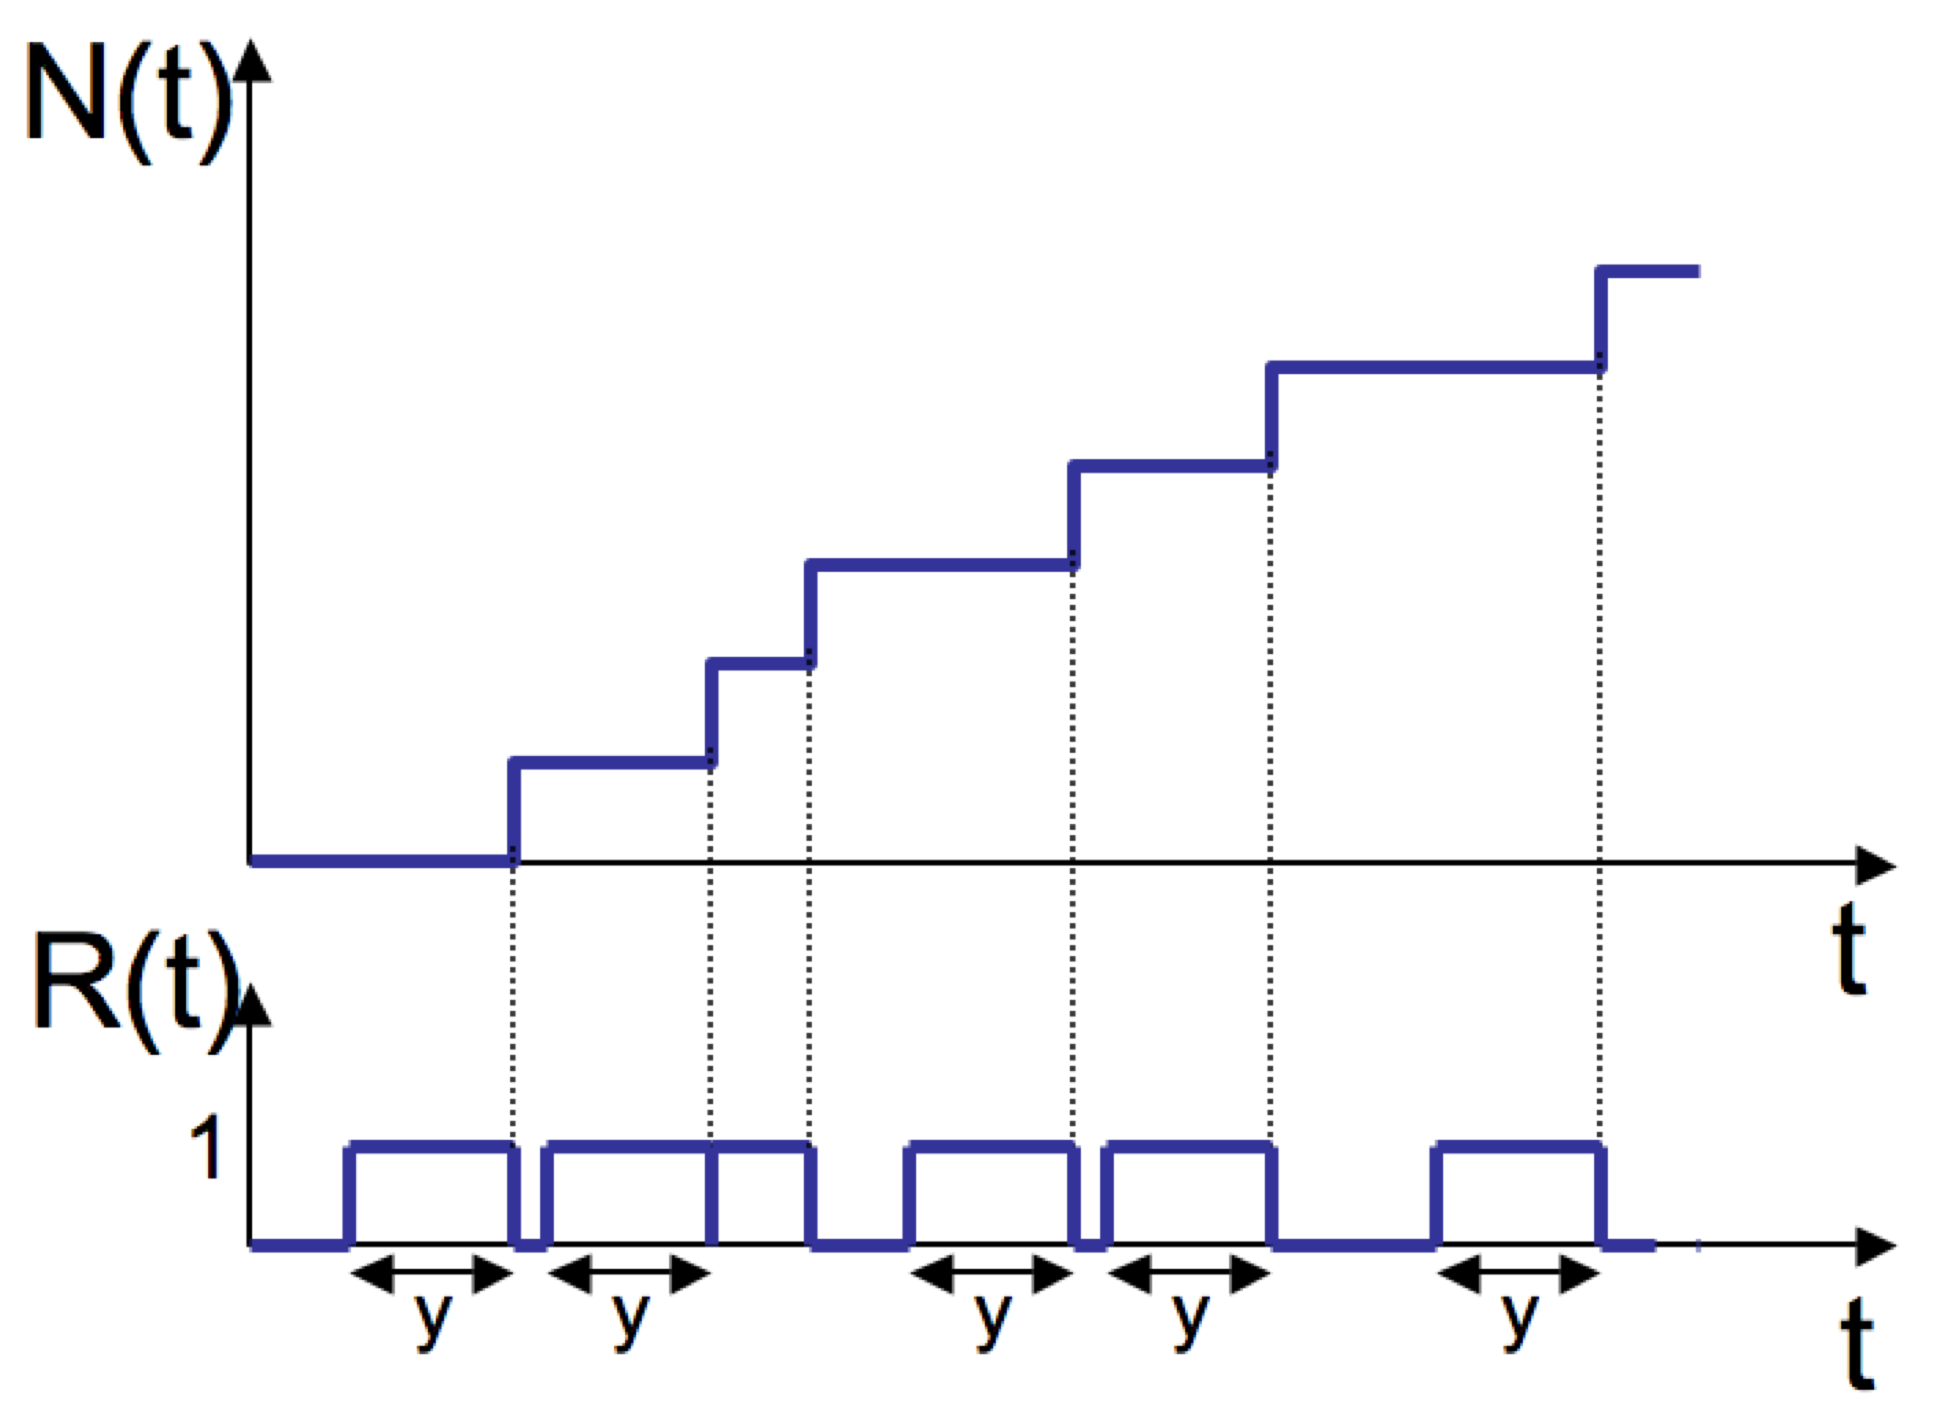
\includegraphics[width=0.5\textwidth]{img/residual.png}
\end{figure}
And we can calculate that 
\begin{equation}
	\begin{aligned}
		\E[R_n]= \int_0^y P[X>x]dx \\
		F_Y(y) = \frac{1}{\E[X]}\int_0^y P[X>x]dx
	\end{aligned}
\end{equation}
\subsection{Key theorem}
Let $N(t)$ be a non-arithmetic renewal process, let $R(z,x)\ge 0$ be such that $r(z)=\int_{x=z}^\infty R(z,x)dF_X(x)$ is directly Rieman integrable. Then, 
\begin{equation}
	\lim_{t\to \infty} \E[R(t)] = \frac{\E[R_n]}{\bar X}
\end{equation}
\section{Little's Law}
Let a queueing system be such that 
\begin{itemize}
	\item $A(t)$ is the number of arrivals between $0$ and $t$;
	\item $D(t)$ is the number of departures between $0$ and $t$;
	\item $L(t)=A(t)-D(t)$ is the number of customers in the system at time $t$;
	\item $w_i$ the time the $i^{th}$ customer spends in the system;
	\item $N(t)$ is the renewal process counting the number of busy periods of the system (each time a customer arrives when the system is empty).
\end{itemize}
\begin{figure}[H]
	\centering
	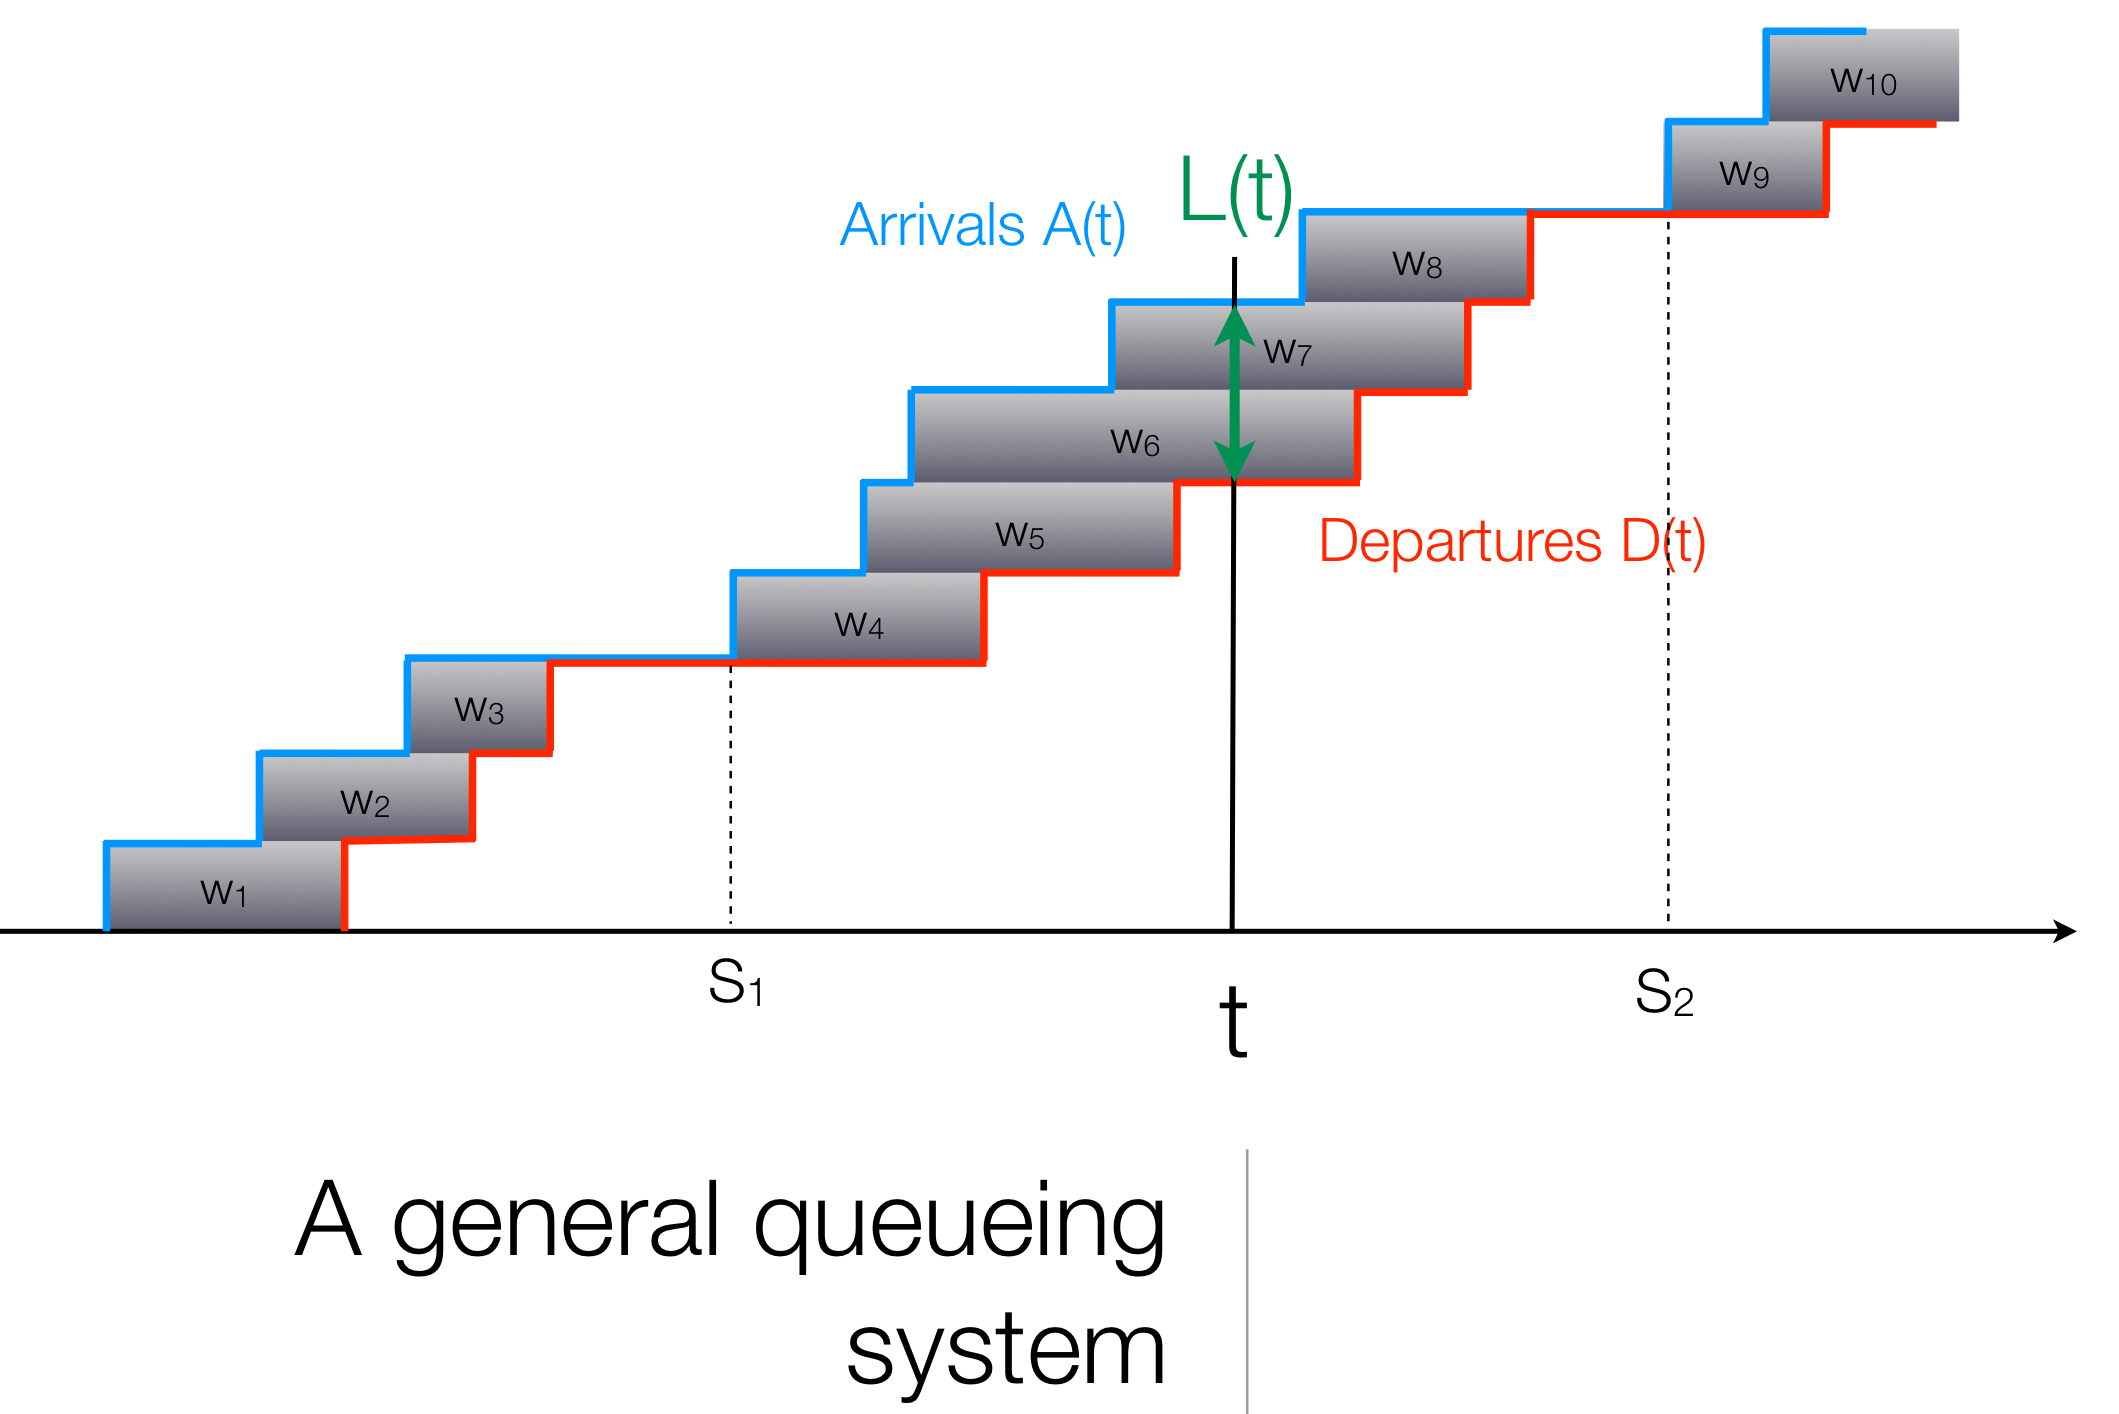
\includegraphics[width=0.5\textwidth]{img/queue.png}
\end{figure}
Let us use $L(t)$ as a reward function for the renewal process $N(t)$. This implies 
\begin{equation}
	\begin{aligned}
		\sum_{n=1}^{N(t)} R_n \le \int_0^t L(\tau)d\tau &\le \sum_{i=1}^{A(t)} w_i \le \sum_{n=1}^{N(t)+1} R_n\\
		\lim_{t\to \infty} \frac{1}{t}\int_0^t L(\tau)d\tau &= \frac{\E[R_n]}{\E[X]}	
	\end{aligned}
\end{equation}
Putting all this together, we can show that $\bar L=\lim_{t\to \infty}\frac{1}{t}\int_0^tL(\tau)d\tau = \bar  W\lambda$.
\subsection{M/G/1 queue}
Let $R(t)$ be the remaining time for the customer being served. Let $U(t)$ be the time an arrival at time $t$ would have to wait before being served. Let $L_q(t)$ be the number of customers in queue at time $t$, independent of the $Z_i$. We define 
\begin{equation}
	U(t)=\sum_{i=1}^{L_q(t)}Z_i + R(t) \Longrightarrow \E[U(t)]=\E[L_q(t)]\E[Z]+\E[R(t)]
\end{equation}
We can show that 
\begin{equation}
	\int_0^{S_N(t)} R(\tau)d\tau \le \int_0^{S_N(t)+1} R(\tau)d\tau
\end{equation}
And from Little's Law,
\begin{equation}
	\lim_{t\to \infty} \E[L_q(t)] = \lambda \bar W_q \Longrightarrow \lim_{t\to \infty} \E[U(t)] = \lambda \bar W_q \E[Z] + \lambda \frac{\E[Z^2]}{2} 
\end{equation}
Poisson arrival process implies that arrivals occur with identical probability at any moment, this implies independence with $U(t)$. Hence $\E[W_q(t)]=\E[U(t)]$. Hence $\bar W_q = \lambda \bar W_q\E[Z] + \lambda \frac{\E[Z^2]}{2}$. And we can isolate $\bar W_q$:
\begin{equation}
	\bar W_q = \frac{\lambda (\E[Z]^2+\sigma^2)}{2(1-\lambda \E[Z])}
\end{equation}
And we remember $\bar W = \bar W_q + \E[Z]$.\\
\chapter{Finite State Markov Chains}
\section{Definitions}
A Markov chain is a stochastic process with fixed intervals $\{X_n,n\ge 0\}$ such that each random variable $X_n,n\ge 1$ depends on the past only through the most recent random variable $X_{n-1}$:
\begin{equation}
	P[X_n=j|X_{n-1}=i, X_{n-2}=k,\dots,X_0=m] = P[X_n=j|X_{n-1}=i] = P_{ij}
\end{equation}
The rv $X_n$ is called the state of the Markov chain, and the set of possible sample values for the states lie in a countable set. A Markov chain can be represented under a graph or matrix form:\\
\begin{minipage}{.5\textwidth}
	\begin{figure}[H]
		\centering 
		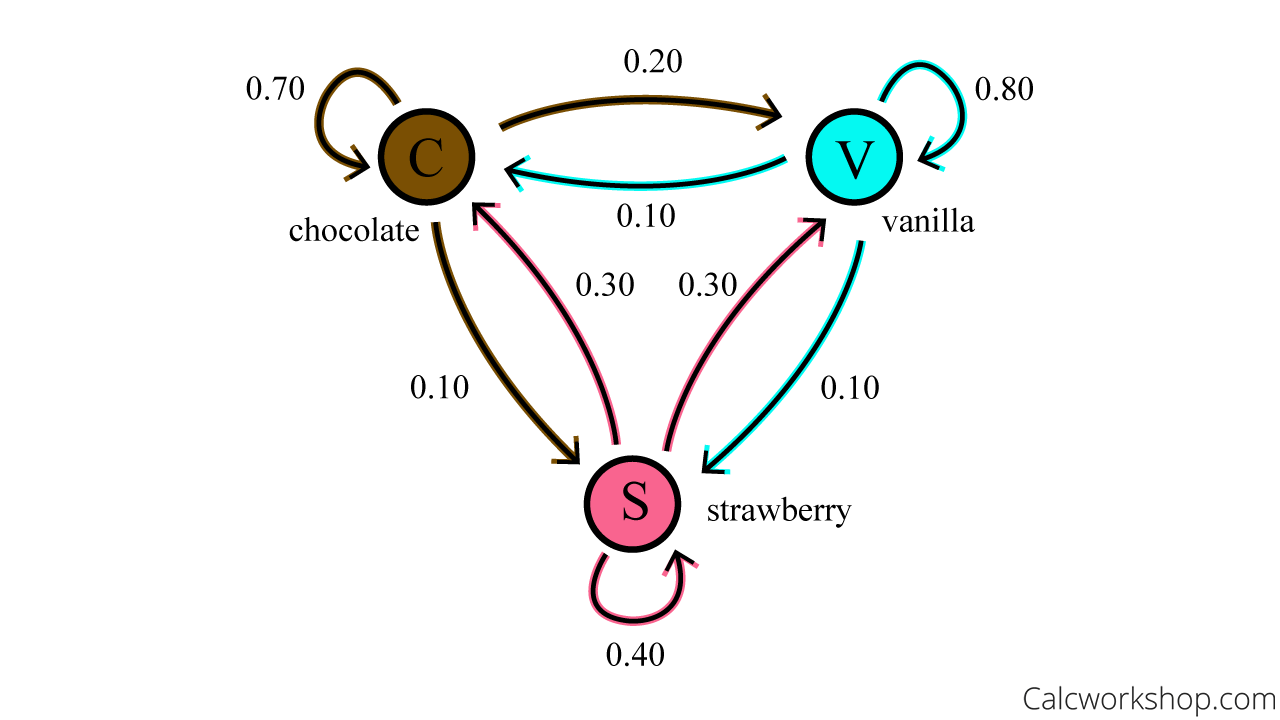
\includegraphics[width=\textwidth]{img/markov_graph.png}
	\end{figure}
\end{minipage}
\begin{minipage}{.5\textwidth}
	\begin{equation}
		P = \begin{pmatrix}
		0.70 & 0.20 & 0.10 \\
		0.10 & 0.80 & 0.10 \\
		0.30 & 0.30 & 0.40 \\
		\end{pmatrix}
	\end{equation}
\end{minipage}
\begin{itemize}
	\item We say that a state $j$ is accessible from $i$ ($i\to j$) if there exists a xalk in the graph from $i$ to $j$: $i\to j$ iff $P_{ij}^n = P[X_n=j|X_0=i]>0$ for some $n$.
	\item Two distinct states $i,j$ communicate ($i\leftrightarrow j$) if $i$ is accessible from $j$ and vice versa. 
	\item A class $C$ of states is a non-empty set of states such that for each $i\in C$, each state $j\neq i$ satisfies $j\in C$ if $i\leftrightarrow j$ and $j\not \in C$ if $i\not \leftrightarrow j$.
	\item A state $i$ is recurrent if it is accessible from all states that are accessible from $i$. A transient state is a state that is not recurrent.
	\item [$\to$] Note: all states of a same class are of the same type.
	\item A finite-state Markov chain has at least one recurrent class.
	\item The period of a state $i$, denoted $d(i)$, is the greatest common divisor of all $n$ such that $P_{ii}^n>0$. A state is aperiodic if $d(i)=1$.
	\item [$\to$] Note: All states of a class have the same periodicity.
	\item If a class has a period $d>1$, then there existsa  partition $\{C_i\}_{i=1}^d$ of the states of the class such that all the transitions from a state of $C_n$ go to a state of class $C_{n+1}$ and all transitions from $C_d$ go to a state of $C_1$, i.e. we make a cycle of subclasses. 
	\item A class is called ergodic if it is aperiodic and recurrent.
	\item A matrix is stochastic iff it is square, non negative ad each row sums to 1, i.e. $P\mathbb{1}_n=\mathbb{1}_n$. 
\end{itemize}
\section{Transition probabilities}
We can calculate that 
\begin{equation}
	P[X_{n+2}=j|X_n=i] = P_{ij}^2 = \sum_{k=1}^J P_{ik}P_{kj} \Longrightarrow P^2 = P\cdot P \Longrightarrow P^n = P\cdot... \cdot P
\end{equation}
More generally, $P_{ij}^{n+m} = \sum_{k=1}^J P_{ik}^nP_{kj}^m$.\\
Because of ergodicity, all rows converge to the same value, and we store those values in a row vector called $\pi$. Then, $\pi = \pi P$ and the sum of all values of $\pi$ is 1.\\ 

From this, we induce that $\pi$ is a left eigenvector of $P$ for the eigenvalue $1$, and the number of linearly independent solutions corresponds to the multiplicity of the eigenvalue $1$. There will be one independent solution for each recurrent class of $P$. Moreover, if $P$ is ergodic, then $\displaystyle \lim_{n\to \infty} P^n = \mathbb{1}_m \pi$, else $\pi$ will be the average over the different subclasses. \\
\section{Markov chains with rewards}
Let $r_i$ be the reward associated with state $i$. In the case where the reward is on the edge from node $i$ to $j$ and not the states, the reward is $r_{ij}$ and we have $\displaystyle r_i = \sum_j P_{ij}r_{ij}$. For an ergodic chain, we observe that the average reward per period will be 
\begin{equation}
	g = \sum_i r_i\pi_i
\end{equation}
where $\pi_i$ is the steady state probability. 
\subsection{Expected reward over multiple transitions}
Let $X_m$ be the state at time $m$ and let $R_m=R(X_m)$ be the reward at time $m$. Under the condition $X_m=i$ (starting point), the aggregate expected reward $v_i(n)$ over $n$ periods from $X_m$ to $X_{m+n-1}$ is 
\begin{equation}
	v_i(n) = \E[R(X_m) + \dots + R(X_{m+n-1})|X_m = i] = r_i + \sum_j P_{ij}r_j + \dots + \sum_j P_{ij}^{n-1}r_j
\end{equation}
And in vector notation 
\begin{equation}
	v(n) = r+ [P]r + \dots + [P^{n-1}]r = \sum_{h=0}^{n-1}[P^h]r
\end{equation}
\subsection{Relative gain vector}
Assuming the Markov chain is an ergodic unichain, i.e. it has a single ergodic class with possibly some transient classes, we know that $\lim_{n\to \infty}[P^n] = \mathbb{1}_m \pi$ and thus 
\begin{equation}
	\lim_{n\to \infty} [P^n]r = \mathbb{1}_m \pi r = g\mathbb{1}_m 
\end{equation}
This means that the expected reward per period converges to $g$. From this, we can evaluate the transient effect and define the relative-gain vector, denoted by $w$:
\begin{equation}
	w = \lim_{n\to \infty}(v(n)-ng\mathbb{1}_m) = \lim_{n\to \infty}\sum_{h=0}^{n-1} [P^h-\mathbb{1}_m\pi]r
\end{equation}
It can also be computed by solving the following equations instead of calculating the limit:
\begin{equation}\label{eq:rel_gain}
	w+g\mathbb{1}_m = [P]w + r \qquad \pi w=0
\end{equation}
The second equation means that the sum (weighted by the probabilities) of all gains is 0.
\section{Markov decision processes}
Suppose that in each state $i$, we can choose between $K_i$ different possibilities with rewards $r_i^{(1)},\dots,r_i^{(K_i)}$. This means that we choose between different Markov chains that have the same states but not necessarily the same edges. We want to find the optimal (stationary or dynamic) policy for this problem. 
\subsection{Dynamic programming algorithm for the dynamic optimal policy}
This section aims to find a dynamic programming algorithm for the dynamic optimal policy. We assume here that for any policy $A$, the resulting Markov chain with matrix $[P^A]$ is an ergodic unichain.\\

Let $v(0)$ be the final reward vector. Through a recurrence method, we can show that 
\begin{equation}
	v_i^*(n) = \max_k \{r_i^{(k)}+\sum_j P_{ij}^{(k)}v_j^*(n-1)\}
\end{equation}
or in vector form:
\begin{equation}
	v^*(n) = \max_A \{r^A + [P^A]v^*(n-1)\}
\end{equation}
for a policy $A$, i.e. a decision $k_i$ for each state $i$. From equations \eqref{eq:rel_gain}, we know that 
\begin{equation}
	w^A = r^A - g^A\mathbb{1}_m + [P^A]w^A
\end{equation}
and thus 
\begin{equation}
	v^A(n) = ng^A\mathbb{1}_m + w^A + [P^A]^n (v(0)-w^A)
\end{equation}
If $v(0)=w^B$ for a policy $B$ such that 
\begin{equation}
	r^B + [P^B]w^B \ge r^A +[P^A]w^A \quad \forall A
\end{equation}
then $B$ is the dynamic optimal policy for each time period, and 
\begin{equation}
	v^*(n) = w^B + ng^B\mathbb{1}_m
\end{equation}
This relation is an equivalence. 
\subsection{Policy improvement algorithm}
\begin{algorithm}
	\caption{Policy improvement algorithm}
	\begin{algorithmic}[1]
		\State \textbf{Step 1:} Choose an arbitrary policy $B$;
		\While{$\exists A\ : \ r^B +[P^B]w^B\stackrel{\le}{\neq} r^A + [P^A]w^B$}
		\State \textbf{Step 2:} Compute $w^B$;
		\State \textbf{Step 3:} Find $A$ such that $r^A + [P^A]w^B \stackrel{\neq}{\ge} r^B +[P^B]w^B$;
		\State \textbf{Step 4:} $B\gets A$;
		\EndWhile
	\end{algorithmic}
\end{algorithm}
\begin{thm}
	Assuming for any policy $A$ that the Markov chain $[P^A]$ is an ergodic unichain, if $B$ is an optimal stationary policy, then 
	\begin{equation}
		\lim_{n\to \infty} v^*(n) - ng^B\mathbb{1}_m = w^B + (\beta - \pi^B w^B)\mathbb{1}_m
	\end{equation}
	\textcolor{red}{What is $\beta$?}
\end{thm}
\section{Dynamic programming algorithm for the stationary optimal policy}
\begin{algorithm}
	\caption{Dynamic programming algorithm for the stationary optimal policy}
	\begin{algorithmic}[1]
		\State \textbf{Step 1:} Fix an arbitrary vector $v(0)$;
		\While{l < u}
		\State \textbf{Step 2:} Compute 
		\begin{equation}
			l = \min_i [v_i^*(n)-v_i^*(n-1)] \qquad u = \max_i [v_i^*(n)-v_i^*(n-1)]
		\end{equation}
		\EndWhile
		\State $l=u=g^A$ and $A$ is the optimal stationary policy.
	\end{algorithmic}
\end{algorithm}
\chapter{Markov Decision Processes and Reinforcement Learning}
\section{MDP and Policies}
\subsection{Markov Decision Process}
A Markov Decision Process models a sequential decision-making process under uncertainty, where moving to the next stage only depends on the current action-state pair.
\begin{definition}
	A Markov Decision Process (MDP) is defined by 
	\begin{itemize}
		\item a set of system states $S$;
		\item a set of actions $\mathcal{A}$;
		\item a set of rewards $R$;
		\item probabilities $p(s',r|s,a)$ of getting a reward $r$ and moving to state $s'$ if action $a$ is taken in state $s$.
	\end{itemize}
	The MDP is finite if the three sets are finite. 
\end{definition}
\begin{figure}[H]
	\centering 
	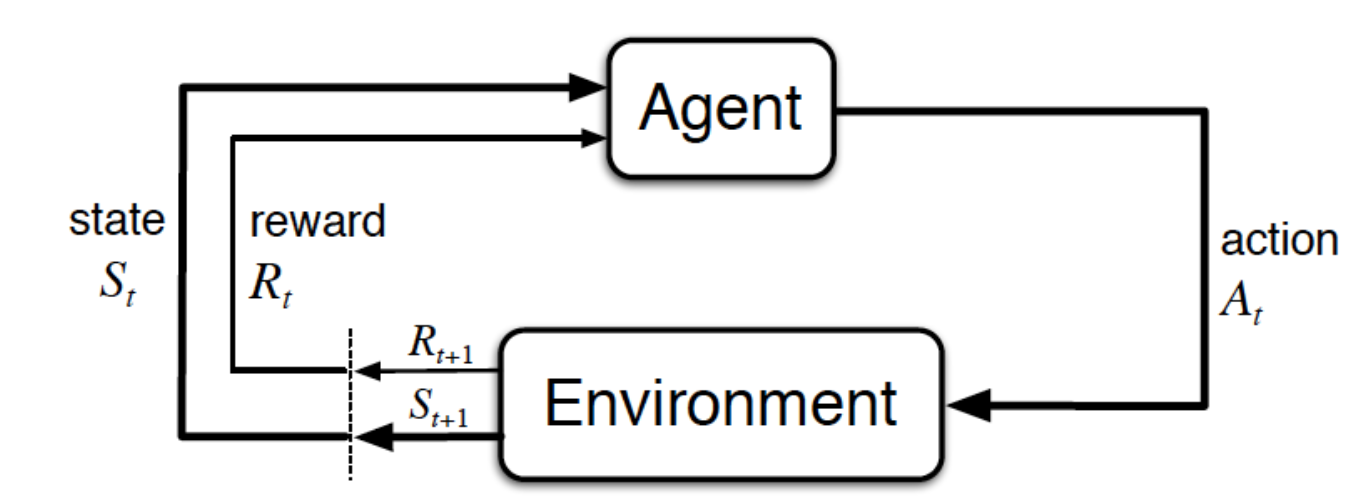
\includegraphics[width=.6\textwidth]{img/MDP.png}
\end{figure}
From the definition, we can derive 3 quantities:
\begin{itemize}
	\item Transition probabilities: $p(sé|s,a) = \sum_r p(s',r|s,a)$;
	\item Reward probabilities: $p(r|s,a) = \sum_{s'}p(s',r|s,a)$;
	\item Expected reward knowing $s,a$: $r(s,a) = \E[R|s,a] = \sum_rr\sum_{s'}p(s',r|s,a)$.
\end{itemize}
\subsection{Policies}
A policy defines the decision making in each state;
\begin{definition}
	A policy is a mapping $\pi:s\in S\to \pi(a|s)$, where $\pi(a|s)$ represents the probability of taking action $a$ in state $s$.
\end{definition}
\subsection{Policy values and state-action values}
The policy value $v_\pi(s)$ at a given state $s$ corresponds to the expected rewards collected over time by applying policy $\pi$ starting from state $s$. 
\begin{equation}
	v_\pi(s) = \E_\pi \left[\sum_{k=0}^\infty \gamma^k R_{t+k+1}|S_t=s\right] 
\end{equation}
where $\gamma \in [0,1[$ is a discounted factor. The state-action value function is the same idea, but has a dependance on the action we intend to take.
\begin{equation}
	q_\pi(s,a) = \E_\pi \left[\sum_{k=0}^\infty \gamma^k R_{t+k+1}|S_t=s,A_t=a\right]
\end{equation}
We can show that 
\begin{equation}
	v_\pi(s) = \E_{A\sim \pi(a|s)}[q_\pi(s,A)]
\end{equation}
Those definitions induce the Bellman equations, a linear system in $v_\pi(s)$:
\begin{equation}\label{eq:bellman}
	\forall s\in S,\quad v_\pi(s) = \sum_a \pi(a|s) \sum_{s'|r}p(s',r|s,a)[r+\gamma v_\pi(s')]
\end{equation}
\subsection{Policy evaluation}
Given the policy $\pi$ and the MDP probabilites $p$, we can rewrite the Bellman equations as 
\begin{equation}
	V=R+\gamma PV \Longleftrightarrow (I-\gamma P)V = R
\end{equation}
where $I-\gamma P$ is invertible as $\|P\|_\infty \le 1$ and $\gamma < 1$. \\
Another way to solve this is by an iterative process: introducing the linear operator $L:V\to \gamma PV+R$, we want to find $V$ such that $V\approx L(V)$. This appraoch is guaranteed to converge since $L$ is $\gamma$-Lipschitz (affine application). Defining $V^* = \lim_{t\to \infty} L^t(V_0)$, with $V_0$ the first iterate, we can show that 
\begin{equation}
	\|V^*-V_{n+1}\|_{\infty} \le \frac{\gamma}{1-\gamma}\|V_{n+1}-V_n\|_\infty 
\end{equation}
\begin{algorithm}[H]
	\caption{Policy Evaluation Algorithm}
	\begin{algorithmic}[1]
		\State \textbf{Input:} $\pi$ the policy to be evaluated, and $\theta$ the guaranteed accuracy of estimation
		\State \textbf{Initialization:} $V(s)$ the arbitrary initial value for all $s$ 
		\While {$\Delta \ge \theta$}
		\State $\Delta =0$
		\For {each state $s$}
		\State $v = V(s)$
		\State $V(s) = \sum_a\pi(a|s)\sum_{s',r} p(s',r|s,a)[r+\gamma V(s')]$
		\State $\Delta = \max(\Delta, |v-V(s)|)$
		\EndFor
		\EndWhile
	\end{algorithmic}
\end{algorithm}
\section{Optimizing Policies}
\subsection{Policy Improvement Theorem}
\begin{thm}
	\begin{equation}
		\left[\forall s\in S,\ q_\pi(s,\pi^{new}(s)) \ge q_\pi(s,\pi(s)) \right] \Longrightarrow v_{\pi^{new}}(s)\ge v_\pi(s)
	\end{equation}
	A strict inequality on the left implies a strict one on the right too. This theorem means that a new policy will be at least as good as a given policy $\pi$ if changing any action of $\pi$ by the corresponding action of $\pi^{new}$ yields a better total gain at the end. 
\end{thm}
\subsection{Bellman optimality conditions}
\begin{definition}
	A policy $\pi^*$ is optimal if for any state $s \in S$ and any other policy $\pi$, $v_{\pi^*}(s)\ge v_\pi (s)$.
\end{definition}
\begin{thm}
	A policy $\pi$ is optimal iff for any state action pair $(s,a)$ with a positive probability to be selected by the policy, i.e. $\pi(a|s)>0$, we have 
	\begin{equation}
		a\in \arg\max_{a'\in A}q_\pi(s,a')
	\end{equation}
	Meaning that any action with a nonzero probability to be taken maximizes the gain of the state at which it is taken.\\
	It can be shown that this implies that any finite MDP admits an optimal policy which is deterministic. 
\end{thm}
This theorem yields the two following equations for optimal policies:
\begin{equation}\label{eq:bellman}
	\begin{aligned}
		v_*(s) &= \max_a q_{\pi^*}(s,a) = \max_{a\in A(s)}\sum_{s',r}p(s',r|s,a)(r+\gamma v_*(s'))\\
		q^*(s,a) &= \sum_{s',r}p(s',r|s,a)(r+\gamma \max_{a'}q^*(s',a'))
	\end{aligned}
\end{equation}
\section{Value Iteration Algorithm}
In the same idea as we did in the evaluation section, let us define the operator $\Phi:V\to \Phi(V)$ such that 
\begin{equation}
	\Phi(V)(s) \coloneqq \max_{a\in A(s)} \sum_{s',r}p(s',r|s,a)(r+\gamma V(s'))
\end{equation}
And thus the Bellman optimality equation (\eqref{eq:bellman}) is equivalent to $V=\Phi(V)$, which can be solved iteratively from the starting point $V_0$. This method is guaranteed because $\Phi$ is a contracting operator ($\sim$ L-Lipschitz function). 
\begin{algorithm}
	\caption{Value Iteration Algorithm}
	\begin{algorithmic}[1]
		\State \textbf{Input: } the guaranteed accuracy of estimation $\theta$;
		\State \textbf{Initialization: } $V(s)\coloneqq$ an arbitrary initial value for all $s$;\\ 
		\quad \qquad \qquad \qquad $\Delta \ge \theta$;
		\While {$\Delta \ge \theta$}
		\State $\Delta = 0$;
		\For {each state $s$}
		\State $v=V(s)$
		\State $V(s) = \max_a \sum_{s',r}p(s',r|s,a)(r+\gamma V(s'))$;
		\State $\Delta = \max (\Delta, |v-V(s)|)$;
		\EndFor
		\EndWhile
	\end{algorithmic}
\end{algorithm}
\end{document}